%%%%%%%%%%%%%%%%%%%%%%%%%%%%%%%%%%%%%%%%%
% Awesome Resume/CV
% XeLaTeX Template
% Version 1.1 (9/1/2016)
%
% This template has been downloaded from:
% http://www.LaTeXTemplates.com
%
% Original author:
% Claud D. Park (posquit0.bj@gmail.com) with modifications by
% Vel (vel@latextemplates.com)
%
% License:
% CC BY-NC-SA 3.0 (http://creativecommons.org/licenses/by-nc-sa/3.0/)
%
% Important note:
% This template must be compiled with XeLaTeX, the below lines will ensure this
%!TEX TS-program = xelatex
%!TEX encoding = UTF-8 Unicode
%
%%%%%%%%%%%%%%%%%%%%%%%%%%%%%%%%%%%%%%%%%

%----------------------------------------------------------------------------------------
%   PACKAGES AND OTHER DOCUMENT CONFIGURATIONS
%----------------------------------------------------------------------------------------

\documentclass[12pt, a4paper]{awesome-cv} % A4 paper size by default, use 'letterpaper' for US letter

\geometry{left=2cm, top=1.5cm, right=2cm, bottom=2cm, footskip=.5cm} % Configure page margins with geometry

\fontdir[fonts/] % Specify the location of the included fonts

% Color for highlights
\colorlet{awesome}{awesome-concrete} % Default colors include: awesome-emerald, awesome-skyblue, awesome-red, awesome-pink, awesome-orange, awesome-nephritis, awesome-concrete, awesome-darknight
%\definecolor{awesome}{HTML}{CA63A8} % Uncomment if you would like to specify your own color

% Colors for text - uncomment and modify
%\definecolor{darktext}{HTML}{414141}
%\definecolor{text}{HTML}{414141}
%\definecolor{graytext}{HTML}{414141}
%\definecolor{lighttext}{HTML}{414141}

\renewcommand{\acvHeaderSocialSep}{\quad\textbar\quad} % If you would like to change the social information separator from a pipe (|) to something else

% ----------------------------------------------------------------------------------------
%   PERSONAL INFORMATION
%   Comment any of the lines below if they are not required
%----------------------------------------------------------------------------------------

\name{Saksham}{Sharma}
% \address{E-255, Hall 2, Indian Institute of Technology Kanpur, Kanpur,
% 208016}
\address{Indian Institute of Technology Kanpur}
\mobile{(+91) 7755-05-8004}

\email{saksham0808@gmail.com}
\homepage{sakshamsharma.com}
\github{sakshamsharma}
\linkedin{saksham-sharma}
%\skype{skypeid}
%\stackoverflow{SOid}{SOname}
%\twitter{@twit}

\position{Third Year Undergraduate{\enskip\cdotp\enskip}Computer
  Science and Engineering} % Your expertise/fields
%\quote{``Make the change that you want to see in the world."} % A
%quote or statement

\makecvfooter{\today}{Saksham Sharma~~~·~~~Résumé}{\thepage} % Specify the letter footer with 3 arguments: (<left>, <center>, <right>), leave any of these blank if they are not needed

%----------------------------------------------------------------------------------------

% \usepackage{tikz}

\begin{document}

\makecvheader % Print the header

% \tikz[remember picture,overlay]
%   \node[anchor=north east,inner sep=0pt] at (current page.north east)
%     {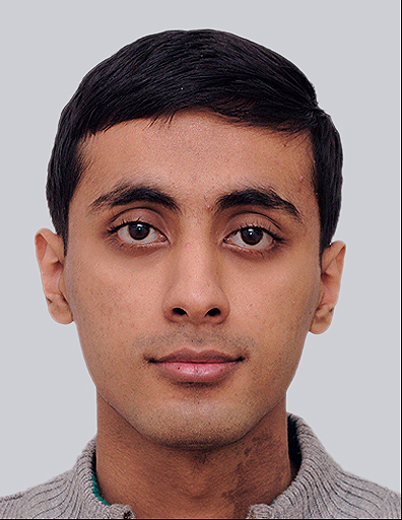
\includegraphics[height=4cm]{me}};

    % ----------------------------------------------------------------------------------------
%   CV/RESUME CONTENT
%   Each section is imported separately, open each file in turn to modify content
%----------------------------------------------------------------------------------------

%----------------------------------------------------------------------------------------
%   SECTION TITLE
%----------------------------------------------------------------------------------------

\cvsection{Education}

%----------------------------------------------------------------------------------------
%   SECTION CONTENT
%----------------------------------------------------------------------------------------

\begin{cventries}

%------------------------------------------------

\cventry
{Bachelor of Technology, major in Computer Science and Engineering} % Degree
{Indian Institute of Technology Kanpur} % Institution
{Kanpur, India} % Location
{2014 - 2018 (Exprected)} % Date(s)
{ % Description(s) bullet points
\begin{cvitems}
\item {Institute Rank 1 among 830 students. Cumulative Grade Point /
    \textbf{CGPA: 10.0/10.0}}
\end{cvitems}
}

\end{cventries}

%%% Local Variables:
%%% mode: latex
%%% TeX-master: "../resume_twopage"
%%% End:

% ----------------------------------------------------------------------------------------
% SECTION TITLE
% ----------------------------------------------------------------------------------------

\vspace{-0.3cm}
\cvsection{Honors \& Awards}

% ----------------------------------------------------------------------------------------
% INTERNATIONAL SUBSECTION
% ----------------------------------------------------------------------------------------

% ------------------------------------------------

\begin{cvhonors}

  % ------------------------------------------------

  \cvhonor
  {President's Gold Medal}
  {For the best academic performance among graduating students}
  {IIT Kanpur}
  {2018}


  %% \cvhonor
  %% {Academic Excellence Award} % Award
  %% {Institute Rank 1 with a GPA of 10/10 in all 8 semesters} % Event
  %% {IIT Kanpur} % Location
  %% {2016} % Date(s)

  % ------------------------------------------------
  \cvhonor
  {Aditya Birla Group Scholarship Awardee}
  {Awarded to 15 students from all IITs}
  {Mumbai}
  {2014}

  \cvhonor
  {All India Rank 10} % Award
  {Joint Entrance Exam Mains, 1.5 million candidates} % Event
  {India} % Location
  {2014} % Date(s)

  % ------------------------------------------------

  \cvhonor
  {All India Rank 138} % Award
  {Joint Entrance Exam Advanced, 150,000 candidates} % Event
  {India} % Location
  {2014} % Date(s)

  \cvhonor
  {Merit Certificate Awardee, Overall \textbf{97.6\%}}
  {Grade 12 national examination}
  {India}
  {2014}

  \cvhonor
  {KVPY Scholarship Awardee}
  {Indian Institute of Science and Government of India}
  {Bangalore}
  {2013}

  \cvhonor
  {NTSE Scholarship Awardee}
  {Government of India}
  {India}
  {2010}

  % ------------------------------------------------

\end{cvhonors}

%%% Local Variables:
%%% mode: latex
%%% TeX-master: "../resume_twopage.tex"
%%% End:

% ----------------------------------------------------------------------------------------
% SECTION TITLE
% ----------------------------------------------------------------------------------------

\cvsection{Work Experience}

% ----------------------------------------------------------------------------------------
% SECTION CONTENT
% ----------------------------------------------------------------------------------------

\begin{cventries}

  % ------------------------------------------------

  \cventry
  {research Fellow, under Dr. Eva Darulová} % Job title
  {Max Planck Institute for Software Systems} % Organization
  {Saarbrücken, Germany} % Location
  {May. 2016 - Jul. 2016} % Date(s)
  {
    \begin{cvitems}
    \item {Developed and evaluated a Scala tool to rewrite
    mathematical floating-point expressions and increase their
    accuracy using a genetic algorithm.}
    \item {Obtained successful results, improving expression errors by
    $\textasciitilde50\%$, for scientific and embedded
    applications.}
    \item {Part of a larger tool for optimizing numeric expressions,
        will hopefully appear in publication soon.}
    \end{cvitems}
  }

  \cventry
  {Full Stack Developer, under Prof. Manindra Agarwal}
  {New York Office, IIT Kanpur}
  {Kanpur, India}
  {May. 2015 - May. 2016}
  {
    \begin{cvitems}
    \item Adjudged as one of the best interns, while being a freshman
    \item Worked on a scalable application in a polyglot environment
      with an extensive technology stack.
    \item Designed and implemented a full search component
      (ElasticSearch and Angular) from scratch.
    \item Implemented code evaluation, attachment support and
      front-end functionality.
    \item Technology used: Scala with Akka, Node.js with Express,
      Angular with TypeScript, ElasticSearch
    \end{cvitems}
  }

  % ------------------------------------------------
\end{cventries}

%%% Local Variables:
%%% mode: latex
%%% TeX-master: "../resume_twopage"
%%% End:

% ----------------------------------------------------------------------------------------
% SECTION TITLE
% ----------------------------------------------------------------------------------------

\cvsection{Projects}

% ----------------------------------------------------------------------------------------
% SECTION CONTENT
% ----------------------------------------------------------------------------------------

\begin{cventries}

  % ------------------------------------------------

  \cventry
  {Undergraduate Project, Prof. Sandeep Shukla}
  {\href{https://github.com/netsecIITK/moVi}{\entrytitlestyle{moVi: Mobile Video Chat Protocol}}
    \ \ \ \normalfont\href{https://github.com/netsecIITK/moVi}
    {github.com/netsecIITK/movi}}
  {IIT Kanpur}
  {Sept. 2016 - Present}
  {
    \begin{cvitems}
    \item Working on developing a protocol for video communication
      vis-a-vis \href{https://mosh.org/}{Mosh (mobile shell)}.
    \item Using UDP to set up a connection-less and secure channel,
      persistent across network IP and location changes.
    \item Trade-off between video quality, stuttering rate vs network
      resources and reliability required.
    \item Exploring, devising ways for transmitting video
      with minimum requirements, distortion with UDP packets.
    \end{cvitems}
  }

  \cventry
  {Course Project, Prof. Piyush Kurur and
    Prof. Satyadev Nandakumar}
  {\href{https://github.com/pclubiitk/puppy-love}{\entrytitlestyle{Anonymous
        and private pair matching platform}
      \ \ \ \normalfont{\href{https://github.com/pclubiitk/puppy-love}
      {acehack.org/puppy}}}}
  {IIT Kanpur}
  {Oct. 2016 - Present}
  {
    \begin{cvitems}
      \item Designed and in the process of implementing an algorithm
        for fully anonymous matching of couples.
      \item Allows the end users to put zero trust in the server
        (admin), irrespective of code on the backend.
      \item Using homomorphic two party computation (assisted by an
        un-trusted server backend) and asymmetric encryption to
        ensure confidentiality and integrity.
    \end{cvitems}
  }

  \cventry
  {Undergraduate Project, Prof. Sandeep Shukla}
  {\href{https://github.com/sakshamsharma/HTTP-Over-Protocol}{\entrytitlestyle{HOP:
        HTTP proxy for arbitrary protocols}}
    \ \ \ \normalfont{\href{https://github.com/sakshamsharma/HTTP-Over-Protocol}
      {acehack.org/hop}}}
  {IIT Kanpur}
  {Aug. 2016}
  {
    \begin{cvitems}
    \item A proxy to wrap and unwrap arbitrary binary data from/to
      HTTP packets, to bypass possible proxy restrictions.
    \item Stayed in \textbf{top 5} of \textit{Github's trending}
      repositories in C++ on first 2 days of release.
    \end{cvitems}
  }

  \cventry
  {Member, Team Robocon IIT Kanpur, Prof. Bhaskardas Gupta}
  {ABU Robocon 2015, Badminton playing robots}
  {IIT Kanpur}
  {Oct. 2014 - Mar. 2015}
  {
    \begin{cvitems}
    \item Programmed and built 2 semi-autonomous robots
      capable of playing badminton on a standard size court.
    \item Used image processing with OpenCV to detect the shuttle
      and predict the trajectory.
    \item Used Kinect and Stereo Vision to get depth of
      field. Programmed the robot using Arduino run by Odroid.
    \item Finished 11th among 85 teams all over India.
    \end{cvitems}
  }

  \cventry
  {Course Project, Computer Networks, Prof. Sandeep Shukla}
  {\href{https://github.com/sakshamsharma/Network-Implementation}{
      \entrytitlestyle{Network Concepts Implementation}}}
  {IIT Kanpur}
  {Aug. 2016 - Present}
  {
    \begin{cvitems}
    \item Wrote an HTTP Server, an HTTP Proxy and an implementation of
      STCP Protocol using socket programming.
    \end{cvitems}
  }


  \cventry{Consecutive two time hackathon winner}
  {Microsoft code.fun.do hackathon}
  {IIT Kanpur}
  {Jan. 2015, Sept. 2015}
  {
    \begin{cvitems}
    \item An application to parse and plot graphs of implicit
      mathematical functions using C\#.
    \item A platform to learn coding, with a
      custom online judge written in Node.js. National 5th (coding milestone).
    \end{cvitems}
  }

  % ------------------------------------------------
\end{cventries}

%%% Local Variables:
%%% mode: latex
%%% TeX-master: "../resume_twopage"
%%% End:

% ----------------------------------------------------------------------------------------
% SECTION TITLE
% ----------------------------------------------------------------------------------------

\cvsection{Extracurricular Activity}

% ----------------------------------------------------------------------------------------
% SECTION CONTENT
% ----------------------------------------------------------------------------------------

\begin{cventries}

  \extraentry
  {Programming Club, Information Security Group}
  {Coordinator}
  {IIT Kanpur}
  {Apr. 2016 - Apr. 2017}
  {
    \begin{cvitems}
    \item Rewrote, deployed, populated club website \href{http://pclub.in}{pclub.in}
    \item Organize and conduct workshops, lectures on programming topics.
    \item Set problems for and organize various programming contests,
      capture the flag contests on campus.
    \end{cvitems}
  }

  \extraentry
  {Techkriti 2016, IIT Kanpur's National Technical Fest}
  {Software Corner Manager}
  {IIT Kanpur}
  {Dec. 2015 - Mar. 2016}
  {
    \begin{cvitems}
    \item Made an esoteric language based on turing machines for a
      national competition.
    \item Wrote an online judge for a High Performance Computing
      contest run on the Param YUVA II supercomputer.
    \end{cvitems}
  }

  \extraentry{Consecutive two time hackathon winner}
  {Microsoft code.fun.do hackathon}
  {IIT Kanpur}
  {Jan. 2015, Sept. 2015}
  {
    \begin{cvitems}
    \item An application to parse and plot graphs of implicit
      mathematical functions using C\#, for Windows Phone.
    \item A platform to learn coding for Windows Phone, with a
      custom online judge written in Node.js.
    \end{cvitems}
  }

\end{cventries}

%%% Local Variables:
%%% mode: xelatex
%%% TeX-master: "../resume_twopage"
%%% End:

% ----------------------------------------------------------------------------------------
%   SECTION TITLE
% ----------------------------------------------------------------------------------------

\cvsection{Skills}

% ----------------------------------------------------------------------------------------
%   SECTION CONTENT
% ----------------------------------------------------------------------------------------

\begin{cvskills}

  % ------------------------------------------------

  \cvskill
  {Programming}
  {\textit{Proficient: } C/C++, Python, Node.js; \hspace{0.3cm}
    \textit{Experienced: } Scala, Haskell}

  % ------------------------------------------------

  \cvskill
  {Web}
  {Express.js with Node.js, Akka with Scala, JavaScript, TypeScript, Angular}

  % ------------------------------------------------

  \cvskill
  {Operating Systems}
  {Gentoo Linux, Arch Linux, Ubuntu}

  \cvskill
  {Utilities}
  {Linux shell utilities, Git, Docker,
    Kubernetes, GDB, ElasticSearch, \LaTeX, Emacs and Vim}

  % ------------------------------------------------

\end{cvskills}

%%% Local Variables:
%%% mode: latex
%%% TeX-master: "../resume_twopage"
%%% End:

% ----------------------------------------------------------------------------------------
% SECTION TITLE
% ----------------------------------------------------------------------------------------

\cvsection{Coursework}

{\fontsize{11pt}{1em}\bodyfontlight\upshape\color{text}
\begin{tabular*}{\textwidth}{L{0.6cm} L{\textwidth/2 - 1cm} L{0.6cm}
  L{\textwidth/2 - 1cm}}
  A$*$ & Data Structures and Algorithms & A$*$ & Computer Organization\\
  A$*$ & Introduction to Programming & A$*$ & Tools for Computing \\
  A & Computer Systems Security & A & Discrete Mathematics \\
  A & Abstract Algebra, Logic & $i$ & Programs, Proofs and Types \\
  $i$ & Computer Networks & $i$ & Operating Systems
\end{tabular*}
}
{\fontsize{11pt}{1em}\footerfont\upshape\color{text}
\begin{tabular*}{\textwidth}{L{8.4cm} L{3cm} L{3.5cm}}
  \entrylocationstyle{A$*$: Grade for exceptional performance} &
                                                                 \entrylocationstyle{A: grade} & \entrylocationstyle{$i$: In progress}\\
\end{tabular*}
}
\vspace{-0.5cm}

% ----------------------------------------------------------------------------------------
% SECTION CONTENT
% ----------------------------------------------------------------------------------------

%%% mode: xelatex
%%% End:

%%% Local Variables:
%%% mode: latex
%%% TeX-master: "../resume_twopage"
%%% End:

\cvsection{Miscellaneous}

{\fontsize{11pt}{1em}\bodyfontlight\upshape\color{text}
\begin{itemize}
  \item Blog about Networks, Linux, and programming in
    general at \href{http://acehack.org}{acehack.org}
  \item Contribute to open source, maintain some well appreciated
    projects on \href{https://github.com/sakshamsharma}{Github}
  \item Microsoft Build The Shield 2016, National 10th in final,
    on-site Capture The Flag contest.
  \item Administer student servers in IIT Kanpur, including a community Gentoo
    mirror, deploying and managing services for the campus community.
\end{itemize}
}

%%% Local Variables:
%%% TeX-master: "../resume_twopage"
%%% End:


%----------------------------------------------------------------------------------------

\end{document}
%%% Local Variables:
%%% mode: latex
%%% TeX-master: t
%%% End:
